% Set the author and title of the compiled pdf
\hypersetup{
	pdftitle = {\Title},
	pdfauthor = {\Author}
}

\section*{Ordered Binary Trees}

\subsection*{Binary Trees}

Ordered binary trees, also called {\it sorted binary trees} or {\it search
trees} are a data structure commonly used in computer science.

First, let us define some terminology we can use throughout this section:

\begin{description}
	\item {\bf Node}\\ 
		An Object containing data that has zero, one or two links to other nodes.
	\item {\bf Root node}\\
		The node at the top of the tree.
	\item {\bf Child nodes}\\
		Any node can have a left and/or right child, these are linked to the current node.
	\item {\bf Empty node}\\
		A node with no children, sometimes called a leaf of the tree.
	\item {\bf Tree depth}\\
		The maximum number of levels in the tree. A tree with no nodes has a depth of 0.
	\item {\bf Singleton tree}\\
		A tree with only one node. It has a depth of one.
\end{description}

\marginpar{Note that if a node is not empty (i.e. it has one or more children),
it will {\it always} have a left and a right child, even if one of them is
null.}

Here is an example of a binary tree:

\begin{center}
	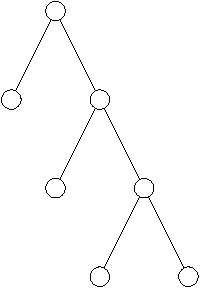
\includegraphics{trees/1.pdf}
\end{center}

\subsection*{Ordering the trees}

However, up to now, we've only looked at trees of generic objects, but when
you're applying trees to real problems, it's often a requirement to have some
sort of ordering. To make things easy, we'll populate our tree with natural
numbers, since they are easy to order, but remember that any object that can be
ordered will do.

\marginpar{In Java, any object that can be ordered usually means an Object that
implements the {\tt Comparable} interface.}

An ordered binary tree with the same structure as the one above, but with actual
data might look like this:

\begin{center}
	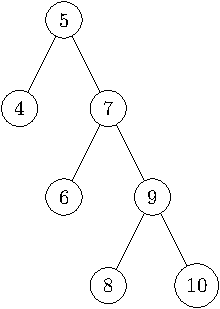
\includegraphics{trees/2.pdf}
\end{center}

The data in the tree is the integers from $4$ through until $10$ (they don't
need to be consecutive as in this example though!).

\subsection*{Why are OBT's useful?}

Ordered Binary Trees are so commonly used because they can be traversed and
searched relatively quickly, especially when compared to a list. In order to
find an item in an OBT, you only ever need to do at most $n$ operations, where
$n$ is the depth of the tree, while with a list, you may need to go through the
whole list before you find the correct item.

Since OBT's are, by definition, sorted, you can use them to sort lists of
objects. If you insert an unordered list of objects into the tree, then when
you've finished inserting, all you need to do it read off the objects from left
to right and you'll get the sorted list.

\subsection*{Balancing trees}

A {\it balanced} tree is one where there is a difference of one between the
number of items on the left of the tree and the number of items on the right.
Any tree can be manipulated so that it is in this form, which is good since it
makes searching the tree a lot faster.

A tree is said to be {\it {\bf fully} balanced} if there are an equal number of
nodes on the left and the right of the tree. This can only happen if the number
of items in the tree is $2^x - 1$ for some $x$. If the tree is fully balanced,
then its depth will always be $log_2(N + 1)$ where $N$ is the number of items
in the tree.

\marginpar{The structure of a tree often depends on the order in which the items
were inserted. For example, if they are inserted in ascending order, then the
tree will have its maximum depth, and basically just be a {\tt LinkedList}}.

\subsection*{Implementing ordered binary trees}

Trees are, by their definition, recursive data structures. If you take any sub
tree from within a tree, then it is also a tree in its own right. That means
that operations on trees are often implemented using recursion.

% Go over the constructor and class structure, then operations.
